\documentclass{beamer}
\mode<presentation>
\usetheme{CambridgeUS}
\usepackage[russian]{babel}
\usepackage[utf8]{inputenc}
\usepackage[T2A]{fontenc}
\usepackage{sansmathaccent}

\usepackage{verbatim}
\usepackage{alltt}

\pdfmapfile{+sansmathaccent.map}
\title[Основы языка Pascal]{Циклические вычислительные процессы}
\author{Наумов Д.А., доц. каф. КТ}
\date[17.10.2019] {Программирование и алгоритмические языки, 2019}

\begin{document}

%ТИТУЛЬНЫЙ СЛАЙД
\begin{frame}
  \titlepage
\end{frame}
  
%СОДЕРЖАНИЕ ЛЕКЦИИ
\begin{frame}
  \frametitle{Содержание лекции}
  \tableofcontents  
\end{frame}

\section{Циклические алгоритмы}

\begin{frame}{Циклические алгоритмы}
Вычислительный процесс с многократным повторением однотипных вычислений для различных значений обрабатываемых величин называется \textbf{циклическим}, повторяющиеся участки вычислений - \textbf{циклами}, изменяющиеся в цикле величины - \textbf{переменными цикла}.

Для организации циклических алгоритмов необходимо предусмотреть:
\begin{enumerate}
\item подготовку цикла: задание начальных значений переменным цикла перед первым его выполнением;
\item тело цикла: действия, повторяемые в цикле для различных значений переменных цикла;
\item модификацию (изменение) значений переменных цикла перед каждым новым его повторением;
\item управление циклом: проверку условия продолжения цикла и переход на начало тела цикла, если условие продолжение выполняется (или выход из цикла, если условие не выполняется).
\end{enumerate}
\end{frame} 

\begin{frame}{Блок-схема циклического алгоритма}
\begin{figure}[h]
\centering
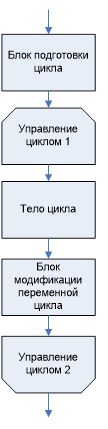
\includegraphics[scale=0.6]{images/lec04-pic01.png}
\end{figure}
\end{frame}

\begin{frame}
Табулирование функции - вычисления значений функции $f$ переменной $х$, изменяющейся от $x_0$ до $x_n$ с постоянным шагом $h$. 
\begin{minipage}{0.6\textwidth}
\begin{flushleft}
\begin{enumerate}
\item подготовка - присвоение переменной х начального значения $x_0$; 
\item тело цикла - вычисление значения функции для очередного значения аргумента и вывод полученного значения; 
\item переменной цикла является переменная x; 
\item модификацией является увеличение значения переменной x на величину шага h;
\item управление цикла - проверка условия (х <= xn).
\end{enumerate}
\end{flushleft}
\end{minipage}
%\hfill
\begin{minipage}{0.2\textwidth}
\begin{flushright}
\begin{figure}[h]
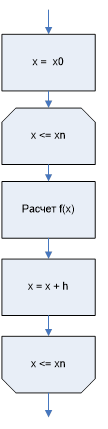
\includegraphics[scale=0.6]{images/lec04-pic02.png}
\end{figure}
\end{flushright}
\end{minipage}
\end{frame}

\begin{frame}{Оператор цикла с параметром}
Различают циклы:
\begin{itemize}
\item с заданным числом повторений;
\item с заранее неизвестным числом повторений. 
\end{itemize}
Циклы первого типа называются \textbf{циклами со счетчиком} или \textbf{циклы с параметром}. 
\begin{enumerate}
\item число повторений такого тела такого цикла подсчитывается с помощью специальной переменной - счетчика, для которой известны начальное и конечное значение, а также шаг ее изменения.
\item переменную-счетчик называют параметром цикла.
\end{enumerate}
\end{frame}

\begin{frame}{Оператор цикла с параметром}
При схематичном изображении цикла с параметром в блок <<Управление циклом 1>> записывается информация в следующей форме:
\begin{itemize}
\item Параметр = Начальное значение (Шаг изменения) Конечное значение
\end{itemize}
Для задачи табулирования функции $f(x)$ переменной $х$, изменяющейся в интервале от $x_0$ до $x_n$ с постоянным шагом $h$, блок <<Управление циклом 1>> будет иметь следующий вид:
\begin{figure}[h]
\centering
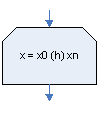
\includegraphics[scale=1]{images/lec04-pic03.png}
\end{figure}
\end{frame}

\begin{frame}[fragile]{Оператор цикла с параметром}
Для программирования циклов с известным числом повторений следует пользоваться оператором цикла с параметром, который имеет следующий вид:
\begin{alltt}
1  for Параметр := Выражение1 to Выражение2 do
2     Оператор
\end{alltt}
или
\begin{alltt}
1  for Параметр := Выражение1 downto Выражение2 do
2     Оператор
\end{alltt}
\begin{itemize}
\item Параметр - переменная порядкового типа
\item Выражение1, Выражение2 - выражения того же типа, что и Параметр 
\item Оператор - оператор языка
\end{itemize}
\end{frame}

\begin{frame}
\begin{minipage}{0.6\textwidth}
\begin{flushleft}
\begin{enumerate}
\item Выражение1 вычисляется до выполнения тела цикла один раз и является блоком подготовки цикла. При помощи данного выражения задается начальное значение переменной цикла.
\item Выражение2 вычисляется в цикле перед выполнением тела цикла и является блоком управления цикла.
\begin{itemize}
\item Параметр <= Выражение 2 для цикла <<to>>
\item Параметр >= Выражение 2 для цикла <<downto>>
\end{itemize}
\item Модификация параметра выполняется после выполнения тела цикла.
\begin{itemize}
\item inc(Параметр) для цикла <<to>>
\item dec(Параметр) для цикла <<downto>>
\end{itemize}
\end{enumerate}
\end{flushleft}
\end{minipage}
%\hfill
\begin{minipage}{0.2\textwidth}
\begin{flushright}
\begin{figure}[h]
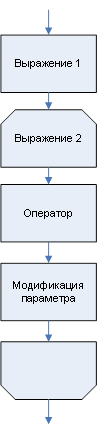
\includegraphics[scale=0.7]{images/lec04-pic04.png}
\end{figure}
\end{flushright}
\end{minipage}
\end{frame}

\begin{frame}{Этапы выполнения цикла for}
\begin{minipage}{0.6\textwidth}
\begin{flushleft}
\begin{enumerate}
\item вычислить значение выражение1; присвоить значение параметру цикла;
\item вычислить выражение2 и условие продолжения цикла;
\item если условие продолжения цикла истинно, то перейти к пункту 4, иначе завершить цикл и перейти к оператору, непосредственно следующему за оператором for
\item выполнить оператор (тело цикла);
\item модифицировать значение параметра цикла;
\item перейти к пункту 2.
\end{enumerate}
\end{flushleft}
\end{minipage}
%\hfill
\begin{minipage}{0.2\textwidth}
\begin{flushright}
\begin{figure}[h]
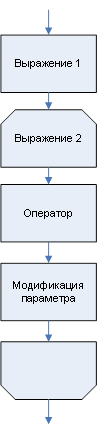
\includegraphics[scale=0.7]{images/lec04-pic04.png}
\end{figure}
\end{flushright}
\end{minipage}
\end{frame}

\begin{frame}{Пример: вычисление степени с натуральным показателем}
Вычислить степень $y = a^n$ действительного числа $a$ с натуральным показателем $n$.
\begin{figure}[h]
\centering
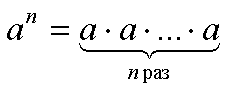
\includegraphics[scale=0.5]{images/lec04-pic05.png}
\end{figure}
Компактно такое произведение может быть записано в следующем виде:
\begin{figure}[h]
\centering
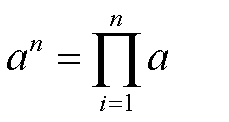
\includegraphics[scale=0.5]{images/lec04-pic06.png}
\end{figure}
\end{frame}

\begin{frame}[fragile]{Пример: вычисление степени с натуральным показателем}
Для вычисления указанного произведения целесообразно организовать цикл с параметром i, в котором осуществлялось бы последовательное накопление произведения y по следующему правилу: 
\begin{itemize}
\item до начала цикла y = 1, 
\item на каждом шаге цикла (для i=1,2,...,n) значение переменной $y$ будет увеличиваться в $a$ раз (то есть y = y * a). 
\item цикл должен быть выполнен n раз (то есть условие цикла $i<=n$).
\end{itemize}
\begin{alltt}
1 var
2   i, n: integer; a, y : extended;
3 begin
4   //ввод a, n
5   y := 1;
6   for i := 1 to n do
7     y := y * a;
8   //вывод y
9 end.
\end{alltt}
\end{frame}

\begin{frame}[fragile]{Пример: вычисление суммы чисел}
Вычислить сумму нечетных чисел, находящихся в интервале от $a$ до $b$. 
\begin{itemize}
\item используем цикл с параметром i от $a$ до $b$
\item в теле цикла следует проверить, что текущее значение параметра цикла нечетным, и если является, то прибавить это значение к переменной s, которая в данной задаче будет использоваться для накопления суммы. 
\item перед началом цикла значение s должно быть нулевым.
\end{itemize}
\begin{alltt}
1 var
2   a, b, i, s: integer;
3 begin
4   //ввод a, b
5   s := 0;
6   for i := a to b do
7     if i mod 2 = 1 then
8        s := s + i;
9   //вывод s
10 end.
\end{alltt}
\end{frame}

\begin{frame}{Табулирование функции}
Вывести на печать значения функции $y = x^2$ для переменной $х$, изменяющейся в интервале от $x_0$ до $x_n$ с постоянным шагом $h$.
\begin{figure}[h]
\centering
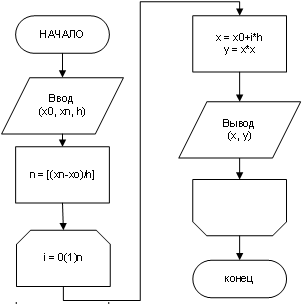
\includegraphics[scale=0.7]{images/lec04-pic07.png}
\end{figure}
\end{frame}

\begin{frame}[fragile]{Пример: вычисление суммы чисел}
Вывести на печать значения функции $y = x^2$ для переменной $х$, изменяющейся в интервале от $x_0$ до $x_n$ с постоянным шагом $h$.
\begin{alltt}
1 var
2   h, x, x0, xn, y: extended; 
3   i, n: integer;
4 begin
5   //ввод x0, xn, h
6   n := round((xn-x0)/h);
7   for i := 0 to n do
8   begin
8     x := x0 + i * h;
9     y := x * x;
10    //вывод x, y
11  end; 
12 end.
\end{alltt}
\end{frame}

\begin{frame}[fragile]{Циклы с неизвестным числом повторений}
Достаточно часто приходится сталкиваться с вычислительными процессами, когда число повторений цикла неизвестно, а задано некоторое условие его окончания (или продолжения). Для программной реализации таких вычислительных процессов существует два типа операторов: 
\begin{itemize}
\item оператор цикла с предусловием 
\item оператор цикла с постусловием.
\end{itemize}
\begin{alltt}
1 while Выражение do
2   Оператор
\end{alltt}
\begin{itemize}
\item while, do - ключевые слова, 
\item Выражение - логическое выражение, 
\item Оператор - любой оператор языка.
\end{itemize}
\end{frame}

\begin{frame}[fragile]
\begin{itemize}
\item Выражение задает условие продолжения цикла
\item Выражение вычисляется перед каждым выполнением цикла (отсюда и термин - предусловие)
\item Если значение Выражения ложно с самого начала, то Оператор не выполнится ни разу.
\end{itemize}
\begin{alltt}
1 while Выражение do
2   Оператор
\end{alltt}
\begin{minipage}{0.6\textwidth}
\begin{flushleft}
Выполнение оператора цикла с предусловием состоит из следующих шагов:
\begin{enumerate}
\item вычислить Выражение. Если значение выражения истинно, то перейти к пункту 2, иначе завершить цикл и перейти к оператору, непосредственно следующему за оператором while. 
\item выполнить оператор (тело цикла);
\item перейти к пункту 1
\end{enumerate}
\end{flushleft}
\end{minipage}
\begin{minipage}{0.2\textwidth}
\begin{flushright}
\begin{figure}[h]
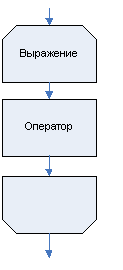
\includegraphics[scale=0.6]{images/lec04-pic08.png}
\end{figure}
\end{flushright}
\end{minipage}
\end{frame}

\begin{frame}[fragile]{Оператор цикла с постусловием}
\begin{alltt}
1 repeat
2   Группа операторов
3 until Выражение
\end{alltt}
\begin{itemize}
\item Выражение задает условие завершения цикла
\item Выражение вычисляется после каждым выполнения цикла
\item Операторы теля цикла выполнятся хотя бы один раз.
\end{itemize}
\begin{minipage}{0.6\textwidth}
\begin{flushleft}
Выполнение цикла с постусловием:
\begin{enumerate}
\item выполнить операторы тела цикла;
\item вычислить Выражение. Если значение выражения ложно, то перейти к пункту 1, иначе завершить цикл и перейти к оператору, непосредственно следующему за оператором repeat-until. 
\item перейти к пункту 1
\end{enumerate}
\end{flushleft}
\end{minipage}
\begin{minipage}{0.2\textwidth}
\begin{flushright}
\begin{figure}[h]
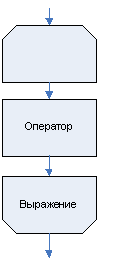
\includegraphics[scale=0.6]{images/lec04-pic09.png}
\end{figure}
\end{flushright}
\end{minipage}
\end{frame}

\begin{frame}{Правило программирования циклов}
\begin{enumerate}
\item перед каждым выполнением цикла условие его продолжения должно быть определено (иметь конкретное значение);
\item тело цикла должно содержать хотя бы один оператор, влияющий на условие продолжения цикла, иначе цикл будет продолжаться бесконечно;
\item условие продолжения цикла должно в конце концов принять значение false;
\item условие вычисляется при каждом выполнении цикла и поэтому должно быть насколько можно простым
\end{enumerate}
\end{frame}

\begin{frame}{Пример. Табулирование функции. Цикл while}
Вывести на печать значения функции $y = x^2$ для $х$ от $x_0$ до $x_n$ с шагом $h$. 
\begin{alltt}
1 var
2   h, x, x0, xn, y: extended; 
3 begin
4   //ввод x0, xn, h
5   x := x0;
6   while x <= xn do
7   begin
8     y := x * x;
9     x := x + h;
10    //вывод x, y
11  end; 
12 end.
\end{alltt}
\end{frame}

\begin{frame}{Пример. Табулирование функции. Цикл repeat-until}
Вывести на печать значения функции $y = x^2$ для $х$ от $x_0$ до $x_n$ с шагом $h$. 
\begin{alltt}
1 var
2   h, x, x0, xn, y: extended; 
3 begin
4   //ввод x0, xn, h
5   x := x0;
6   repeat 
7     y := x * x;
8     x := x + h;
9    //вывод x, y
10  until x > xn; 
11 end.
\end{alltt}
\end{frame}

\begin{frame}{Пример.}
Определить, встречается ли в десятичной записи числа $n$ цифра $d$.
\begin{itemize}
\item нам необходима переменная (зададим ей идентификатор flag), которая будет использоваться как признак того, встретилась ли цифра d при поиске среди цифр десятичной записи числа n.
\item до выполнения основной части алгоритма переменной flag следует присвоить значение false (так как очевидно, что до того, как мы приступили к перебору цифр числа n, цифру d мы еще нашли)
\item необходимо осуществить циклический перебор всех цифр числа d. С точки зрения программирования перебор проще осуществлять, начиная с крайней правой цифры числа. 
\item для того, чтобы получить значение крайней правой цифры числа d, следует вычислить остаток от деления числа d на 10. Затем следует отбросить крайнюю цифру числа (разделив число на 10) и повторять данный процесс до тех пор, пока не будет отброшена последняя цифра (то есть, пока число d не станет равным нулю);
\end{itemize}
\end{frame}

\begin{frame}{Пример.}
Определить, встречается ли в десятичной записи числа $n$ цифра $d$.
\begin{itemize}
\item так как в предыдущей операции производятся математические действия, приводящие к изменению исходных данных (числа, в десятичной записи которого осуществляется поиск заданной цифры), то следует использовать вспомогательную переменную m (присвоив ей после ввода исходных данных значение n), над которой и производить требуемые вычисления.
\item после выполнения перебора всех цифр числа переменная flag будет содержать значение true, если цифра d хотя бы один раз встретилась в десятичной записи числа n, и значение false в про-тивном случае. В зависимости от значения переменной flag следует вывести текстовое сообщение о результатах поиска.
\end{itemize}
\end{frame}

\begin{frame}{Схема алгоритма}
\begin{figure}[h]
\centering
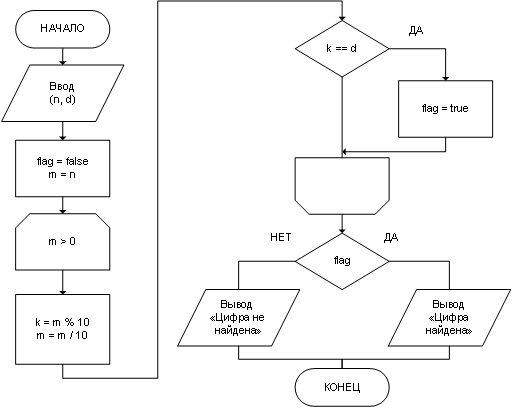
\includegraphics[scale=0.7]{images/lec04-pic10.png}
\end{figure}
\end{frame}

\begin{frame}[fragile]
\begin{alltt}
1 var  
2   d, k, n, m: integer;
3   flag: boolean;
4 begin
5   //ввод n; 
6   //ввод d;
7   m := n;
8   flag := false;
9   while m > 0 do begin
10    k = m mod 10;
11    m = m div 10;
12    if k = d then 
13       flag := true;
14  end;
15  if flag then
16    writeln('число ', n, ' содержит цифру ', d)
17  else
18    writeln('число ', n, ' не содержит цифру ', d);
\end{alltt}
\end{frame}

\begin{frame}[fragile]
\begin{alltt}
1 var  
2   d, k, n, m: integer;
3   flag: boolean;
4 begin
5   //ввод n; 
6   //ввод d;
7   m := n;
8   flag := (n=0) and (d=0);
9   while not flag and (m > 0) do begin
10    k = m mod 10;
11    m = m div 10;
12    if k = d then 
13       flag := true;
14  end;
15  if flag then
16    writeln('число ', n, ' содержит цифру ', d)
17  else
18    writeln('число ', n, ' не содержит цифру ', d);
\end{alltt}
\end{frame}

\section{Вложенные циклы}

\begin{frame}{Вложенные циклы}
Если телом цикла является циклическая структура, то такие циклы называются вложенными или сложными.
\begin{block}{Внешний цикл}
цикл, содержащий в себе другой цикл.
\end{block}
\begin{block}{Внутренний цикл}
цикл, содержащийся в теле другого цикла.
\end{block}
\begin{itemize}
\item Внутренний и внешний циклы могут быть любыми из трех рассмотренных видов: циклами с параметром, циклами с предусловием, циклами с постусловием. 
\item Правила организации как внешнего, так и внутреннего циклов такие же, как и для простого цикла.
\item При построении вложенных циклов необходимо соблюдать следующее дополнительное условие: все операторы внутреннего цикла должны полностью лежать в теле внешнего цикла.
\end{itemize}
\end{frame}

\begin{frame}[fragile]
Сложные циклы условно разбиваются на уровни вложенности.
\begin{minipage}{0.6\textwidth}
\begin{flushleft}
Структура вложенных циклов (рис):
\begin{enumerate}
\item цикл 1 имеет уровень 0;
\item внутренний цикл 2 имеет уровень 1;
\item внутренний цикл 3 имеет уровень 2.
\end{enumerate}
\begin{itemize}
\item Вначале все свои значения изменит параметр цикла наивысшего уровня вложенности при фиксированных (начальных) значениях параметров циклов с меньшим уровнем. 
\item Затем изменяется на один шаг значение цикла предыдущего уровня, и снова выполняется самый внутренний цикл. 
\item Так происходит до тех пор, пока параметры циклов всех уровней не примут все требуемые значения
\end{itemize}
\end{flushleft}
\end{minipage}
\begin{minipage}{0.2\textwidth}
\begin{flushright}
\begin{figure}[h]
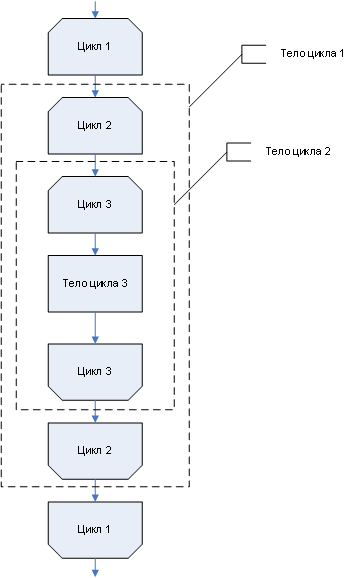
\includegraphics[scale=0.5]{images/lec04-pic11.png}
\end{figure}
\end{flushright}
\end{minipage}
\end{frame}

\begin{frame}{Пример}
Составьте алгоритм и программу вычисления значений функции $z = cos(x) + sin(y)$ для переменных $х = x0 (hx) xn; y = y0 (hy) yn$.
Для определения значений функции z для всех различных пар (x, y) необходимо процесс вычислений организовать следующим образом. 
\begin{itemize}
\item Вначале при фиксированном значении одного из аргументов, например, при х = x0 вычислить значения z для всех заданных y:  y0, y0 + hy, y0+2 hy,..., yn. 
\item Затем, изменив значение x на x+ hx, вновь перейти к полному циклу изменений переменной y.
\end{itemize}
\end{frame}

\begin{frame}[fragile]
\begin{figure}[h]
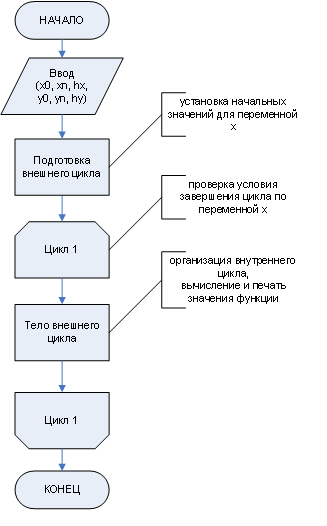
\includegraphics[scale=0.6]{images/lec04-pic12.png}
\end{figure}
\end{frame}

\begin{frame}[fragile]
\begin{figure}[h]
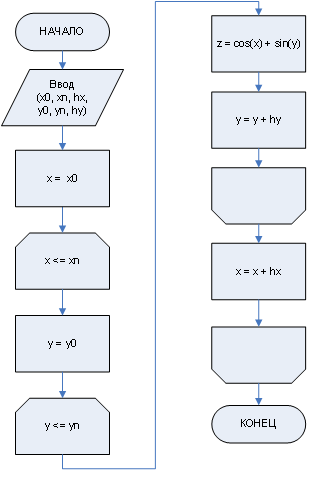
\includegraphics[scale=0.6]{images/lec04-pic13.png}
\end{figure}
\end{frame}

\begin{frame}[fragile]
\begin{alltt}
1 var  
2  x, x0, xn, hx, 
3  y, y0, yn, hy, z: extended;
4 begin 
5 //ввод исходных данных x0, xn, hx, y0, yn, hy
6  x := x0; // подготовка внешнего цикла
7  while x <= xn do begin
8 // подготовка внутреннего цикла
9    y := y0;
10   while y <= yn do begin
       // вычисление значения функции
11     z := cos(x) + sin(y);
12     // вывод x, y, z
       // модификация переменной внутр. цикла
13     y := y + hy;
14   end;
15   x := x + hx;
16 end;
\end{alltt}
\end{frame}

\begin{frame}
Составьте алгоритм и программу вычисления значения выражения: 
\begin{figure}[h]
\centering
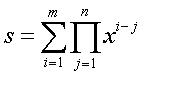
\includegraphics[scale=0.5]{images/lec04-pic14.png}
\end{figure}
s - сумма m слагаемых, каждое слагаемое - произведение из n множителей $x^(i-j)$.

Внутренний цикл будет вычислять значение отдельного слагаемого по формуле:
\begin{figure}[h]
\centering
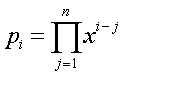
\includegraphics[scale=0.5]{images/lec04-pic15.png}
\end{figure}
а внешний цикл - вычислять значение суммы m слагаемых по формуле:
\begin{figure}[h]
\centering
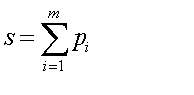
\includegraphics[scale=0.5]{images/lec04-pic16.png}
\end{figure}
\end{frame}

\begin{frame}[fragile]
\begin{figure}[h]
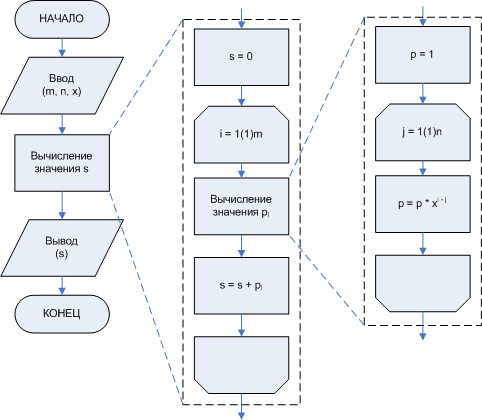
\includegraphics[scale=0.75]{images/lec04-pic17.png}
\end{figure}
\end{frame}

\begin{frame}[fragile]
\begin{alltt}
1 var i, j, m, n: integer;
2     p, s, x: extended;
3 begin
4   //ввод m, n, x
5   s := 0;
6   for i := 1 to m do begin
7     p := 1;
8     for j := 1 to n do 
9       p := p * exp(ln(x) * (i - j));
      s := s + p;
10  end;
11  //вывод s
12 end.  
\end{alltt}
\end{frame}

\begin{frame}{Пример}
Определить количество <<счастливых билетиков>>.

Билет является «счастливым», если в его номере сумма первых трех цифр равна сумме последних трех цифр. Минимальный номер билета – 000 001, максимальный номер билета – 999 999. 

Вариант 1
\begin{itemize}
\item перебрать все возможные номера билетов от 000 001 до 999 999;
\item отделить в номере первые три цифры от последних трех;
\item сравнить сумму первых трех чисел с суммой последних трех чисел, и если суммы совпали, увеличить значение счетчика счастливых билетов.
\end{itemize}
\end{frame}

\begin{frame}[fragile]
\begin{alltt}
1 var  a1, a2, a3, a4, a5, a6: byte; 
2      g, s: longint;
2 begin
3   s = 0;
4   for g := 1 to 999999 do begin
5     a1 := g mod 10;
6     a2 := g div 10 mod 10;
7     a3 := g div 100 mod 10;
8     a4 := g div 1000 mod 10;
9     a5 := g div 10000 mod 10;
10    a6 := g div 100000 mod 10;
11    if a1 + a2 + a3 = a4 + a5 + a6 then s := s + 1;
12  end;
13  writeln('Всего существует ', s, ' счастливых билетов');
14 end.
\end{alltt}
\end{frame}

\begin{frame}{Пример}
Вариант 2
\begin{itemize}
\item организовать внешний цикл – перебор возможных значений цифр первой группы от 000 до 999;
\item организовать внутренний цикл – перебор возможных значений цифр второй группы от 000 до 999;
\item сравнить сумму цифр в числе первой группы с суммой цифр в числе второй группы, и если суммы совпали, увеличить значение счетчика счастливых билетов;
\item учесть, что билета с номером 000 000 не существует.
\end{itemize}
\end{frame}

\begin{frame}{Пример}
Вариант 3
\begin{itemize}
\item организовать шесть вложенных циклов – каждый цикл для перебора значений от 0 до 9, соответствующий одной из цифр шестизначного номера билета;
\item сравнить сумму первых трех чисел с суммой вторых трех чисел, и если суммы совпали, увеличить значение счетчика счастливых билетов;
\item учесть, что билета с номером 000 000 не существует.
\end{itemize}
\end{frame}

\end{document}
